\documentclass[a4paper,12pt]{report}
\usepackage[utf8]{vietnam}
\usepackage{amsmath}
\usepackage{amsfonts}
%\usepackage{enumitem}
\usepackage{enumerate}
%\usepackage{amssymb}
\usepackage{graphicx}
%\usepackage{cases}
\usepackage{fancybox}
\usepackage{multirow}
\usepackage{longtable}
\usepackage{listings}
\usepackage[nottoc]{tocbibind}
\usepackage{indentfirst}
\usepackage[english]{babel}
\usepackage{float}
\PassOptionsToPackage{hyphens}{url}\usepackage{hyperref}  
\usepackage[left=3cm, right=2.00cm, top=2.00cm, bottom=2.00cm]{geometry}
%\lstset{
   %keywords={break,case,catch,continue,else,elseif,end,for,function,
   %   global,if,otherwise,persistent,return,switch,try,while},
%   language = Java,
%   basicstyle=\ttfamily \fontsize{12}{15}\selectfont,   
	% numbers=left,
%   frame=lrtb,
%tabsize=3
%}
\hypersetup{
    colorlinks,
    citecolor=black,
    filecolor=black,
    linkcolor=blue,
    urlcolor=red 
}
%\setlength{\parskip}{0.6em}
\addto\captionsenglish{
 \renewcommand\chaptername{Phần}
 \renewcommand{\contentsname}{Mục lục} 
 \renewcommand{\listtablename}{Danh sách bảng}
 \renewcommand{\listfigurename}{Danh sách hình vẽ}
 \renewcommand{\tablename}{Bảng}
 \renewcommand{\figurename}{Hình}
 \renewcommand{\bibname}{Tài liệu tham khảo}
}

\newtheorem{definition}{Định nghĩa}[chapter]
%\newtheorem{lema}{Bổ đề}[chapter]
%\newtheorem{theorem}{Định lý}[chapter]

\begin{document}
\thispagestyle{empty}
\thisfancypage{
\setlength{\fboxrule}{1pt}
\doublebox}{}

\begin{center}
{\fontsize{16}{19}\fontfamily{cmr}\selectfont TRƯỜNG ĐẠI HỌC BÁCH KHOA HÀ NỘI\\
VIỆN CÔNG NGHỆ THÔNG TIN VÀ TRUYỀN THÔNG}\\
\textbf{------------*******---------------}\\[1cm]

\includegraphics[scale=0.13]{hust.jpg}\\[1.3cm]
{\fontsize{32}{43}\fontfamily{cmr}\selectfont BÁO CÁO}\\[0.1cm]
{\fontsize{38}{45}\fontfamily{cmr}\fontseries{b}\selectfont MÔN HỌC}\\[0.2cm]
{\fontsize{20}{24}\fontfamily{phv}\selectfont Hình học tính t	oán}\\[0.3cm]
{\fontsize{18}{20}\fontfamily{cmr}\selectfont \emph{Đề tài: Lập kế hoạch vận di chuyển cho robot}}\\[2cm]
\hspace{-5cm}\fontsize{14}{16}\fontfamily{cmr}\selectfont \textbf{Nhóm sinh viên thực hiện:}\\[0.1cm] 
\begin{longtable}{l c c}
Nguyễn Tuấn Đạt & 20130856 & CNTT2.02-K58 \\
Phan Anh Tú &   20134501 & CNTT2.01-K58\\
\end{longtable}
\vspace{0.5cm}
\hspace{-6cm}\fontsize{14}{16}\fontfamily{cmr}\selectfont \textbf{Giảng viên hướng dẫn:}\\[0.1cm]
\hspace{-2.7cm}\fontsize{14}{16}\fontfamily{cmr}\selectfont PGS-TS.Huỳnh Thị Thanh Bình \\[3cm]
\fontsize{16}{19}\fontfamily{cmr}\selectfont Hà Nội 5--2017
\end{center}
\newpage
\pdfbookmark{\contentsname}{toc}
\tableofcontents
%\listoftables
%\listoffigures

\chapter{Mở đầu}
Một trong những mục đích cơ bản của ngành robot là thiết kế ra những con robot tự động, những con robot có khả năng tự động lập kế hoạch cho sự di chuyển của nó. Để có thể lập kế hoạch di chuyển, một con robot cần biết về môi trường xung quanh, những trướng ngại vật cần phải tránh. Và bài toán lập kế hoạch di chuyển cho robot là bài toán khó, vì vậy cần có một vài giả sử để làm đơn giản hóa bài toán: 
\begin{itemize}
\item Giả sử bài toán lập kế hoạch vận chuyển cho robot trong không gian hai chiều, với các chướng ngại vật là các đa giác, và robot cũng là một đa giác. 
\item Giả sử môi trường xung quanh robot là tĩnh, tức là không có người đi lại trên đường di chuyển của robot, các chướng ngại vật là cố định.
\end{itemize}


\section{Không gian làm việc, không gian cấu hình}
$R$ là robot di chuyển trong không gian 2 chiều (không gian làm việc), với tập $S = \{P_1, ...., P_t\}$ các chướng ngại vật. Giả sử rằng $R$ là một đa giác. Vị trí của robot có thể định nghĩa bởi một vector. Ta ký hiệu $\mathcal{R}(x,y)$ đại diện cho vector vị trí các đỉnh của robot (Điểm $(x,y)$ được gọi là điểm tham chiếu). Ví dụ robot có các đỉnh: $(1,-1), (1,1), (0,3), (-1,1), (-1,-1)$ thì $\mathcal{R}(6,4)$ sẽ đại diện cho vector vị trí của robot khi các đỉnh đa giác của robot ở các vị trí lần lượt là: $(7,3), (7,5), (6,7), (5,5), (5,3)$\\[0.6em]
Giả sử robot có thể thay đổi hướng của nó thông qua phép quay, vì vậy ta cần định nghĩa thêm một tham số ($\phi$) để biểu diễn hướng của robot. Ký hiệu $\mathcal{R}(x,y,\phi)$ xác định vị trí và hướng của robot, trong đó $(x,y)$ là điểm tham chiếu, $\phi$ là góc quay ngược chiều kim đồng hồ so với vị trí thẳng (vị trí chưa quay của robot)\\[0.6em]
Không gian các tham số của một robot $\mathcal{R}$ thường được gọi là không gian cấu hình ($\mathcal{C}(\mathcal{R})$). Một điểm $p$ trong không gian cấu hình đó sẽ tương ứng với vị trí nào đó $\mathcal{R}(p)$ của robot trong không gian làm việc.
\par Ví dụ điểm $(x,y,\phi)$ trong không gian cấu hình sẽ tương ứng với vị trí $\mathcal{R}(c,y,\phi)$ trong không gian làm việc. Không gian cấu hình là không gian $\mathbb{R}^2\times[0:360)$ (không phải không gian Euclidean 3 chiều) do chiều quay của robot là từ 0 đến 360 độ.
\par Không gian làm việc của là không gian thực tế mà robot di chuyển còn không gian cấu hình là không gian các tham số của robot (điểm tham chiếu, hướng của robot). Một đa giác (hình của robot) trong không gian làm việc sẽ được biểu diễn bởi một điểm trong không gian cấu hình và mọi điểm trong không gian cấu hình tương ứng với một vài vị trí thực của robot trong không gian làm việc.\\[0.6em]
Như vậy bằng cách xác định các giá trị cho các tham số xác định vị trí (hay nói cách khác bằng cách xác định một điểm trong không gian cấu hình) ta có thể xác định được vị trí của robot. Nhưng không phải tất cả các điểm trong không gian cấu hình sẽ xác định vị trí hợp lệ của robot. Đó là các điểm tương ứng với vị trí của các chướng ngại vật trong $S$. Ta gọi phần không gian trong không gian cấu hình chứa các điểm như vậy là không gian cấm (Ký hiệu $\mathcal{C}_{forb}(\mathcal{R},S$). Phần còn lại của không gian cấu hình bao gồm các điểm tương ứng với các vị trí tự do (không vướng các chướng ngại vật) được gọi là không gian tự do (Ký hiệu $\mathcal{C}_{free}(\mathcal{R},S)$).
\par Một đường đi của robot trong không gian làm việc sẽ tương đương với một đường cong trong không gian cấu hình (nối các điểm trong không gian cấu hình tương ứng với các vị trí trên đường đi của robot trong không gian làm việc) (Hình \ref{fig_path})
\begin{figure}[H]
\label{fig_path}
\centering
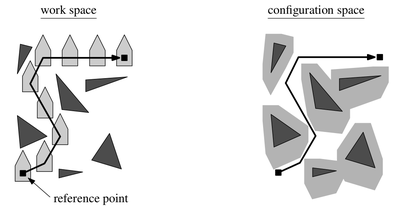
\includegraphics[scale=1]{path.png}
\caption{Đường đi trong không gian làm việc và không gian cấu hình}
\end{figure}
\par Một chướng ngại vật $\mathcal{P}$ trong không gian làm việc tương ứng một tập các điểm $p$ trong không gian cấu hình 


\begin{thebibliography}{9}

\end{thebibliography}


\end{document}
